\section{Simulação Computacional}

Com o objetivo de validar os resultados teóricos obtidos por meio da análise do
circuito, foi realizada uma simulação computacional utilizando o ambiente
Simulink do MATLAB. Essa etapa visa não apenas verificar a coerência dos valores
calculados, mas também proporcionar maior familiaridade com ferramentas de
simulação amplamente utilizadas na engenharia elétrica.

\begin{figure}[H]
  \centering
  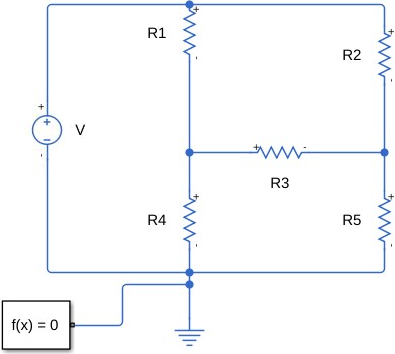
\includegraphics[width=0.5\linewidth]{fig/lab1circuitmatlab.png}
  \caption{Circuito recreado no Matlab}
  \label{fig:circuit-simulink}
\end{figure}

Inicialmente, o circuito foi remontado no Simulink de forma a refletir fielmente
o arranjo teórico. Foram utilizados componentes eletrônicos como resistores,
fontes de tensão e referência elétrica, todos configurados de acordo com os
parâmetros estabelecidos. A Figura~\ref{fig:circuit-simulink} apresenta a
montagem do circuito no ambiente de simulação.

\begin{figure}[H]
  \centering
  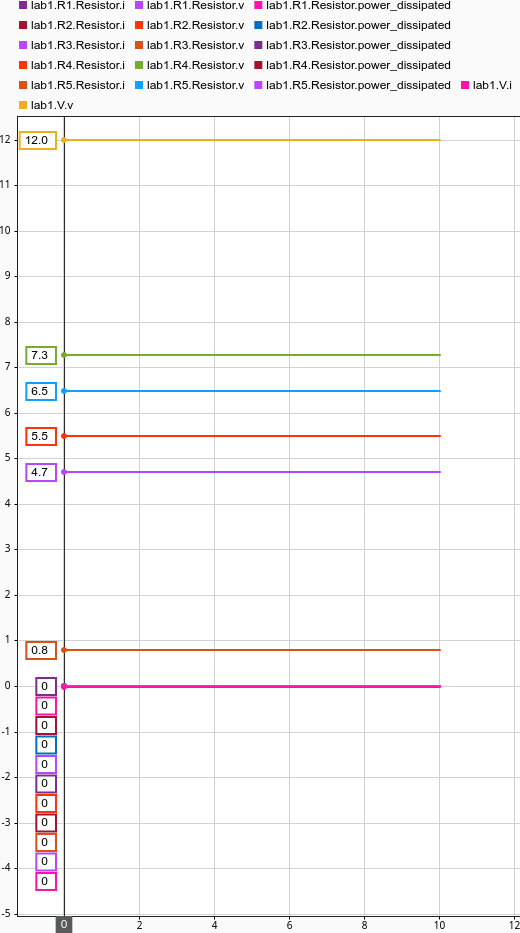
\includegraphics[width=0.7\linewidth]{fig/lab1results.png}
  \caption{Resultados apresentados pelo Matlab}
  \label{fig:simulink-results}
\end{figure}

Após a simulação, os resultados obtidos para as tensões, correntes e potências
nos diversos elementos do circuito foram registrados, conforme ilustrado na
Figura~\ref{fig:simulink-results}. Esses valores foram posteriormente
organizados em tabelas comparativas com os dados teóricos e os dados obtidos em
medições reais. A boa concordância entre os resultados simulados e teóricos
reforça a consistência da análise e evidencia a confiabilidade da simulação como
ferramenta de apoio ao estudo de circuitos elétricos, além da assertividade da
análise realizada por nós.